\documentclass[12pt]{report} % Times New Roman, 12pt
%\usepackage{gscale_thesis_singlespace} % Single spaced thesis
\usepackage{gscale_thesis_doublespace} % Double spaced thesis
\usepackage{fancyheadings} % Header and footer styling
\usepackage{natbib} % Bibliography formatting
\usepackage{setspace} % Allows double spacing but skips headers/footers
\setcounter{tocdepth}{1} % Limits the TOC to chapter and section names

% Additional packages
\usepackage{graphicx} % Allows the inclusion of figures
\usepackage{subcaption} % Allows captions to be added to subfigures
\usepackage[justification=centering]{caption} % Centres caption text
\usepackage{array} % Used for table formatting
\newcolumntype{P}[1]{>{\raggedright\let\newline\\\arraybackslash\hspace{0pt}}m{#1}}
\usepackage{booktabs} % Fancy-style tables
\usepackage{longtable} % Allows for tables that are more than one page long
\usepackage{float} % Better figure placement control
\usepackage{enumerate} % Numbered lists
\usepackage[shortlabels]{enumitem} % For controlling enumerate labels
\usepackage[shortcuts]{extdash} % Allows manual hyphenation of hypenated words
\usepackage{amsmath} % Non-standard math symbols
\usepackage{amsfonts} % Extended fonts for mathematics

\usepackage[hidelinks]{hyperref} % Linking to LaTeX labels and external URLs

\numberwithin{equation}{section} % Numbers equations based on their section

% ********************************
\begin{document}
\title{Reverse Engineering Microservices for Enhanced Insights}
\halftitle{Reverse Engineering Microservices} % 60 Characters Max. Including Spaces

\author{Muhammad Waqar Ul Hassan Awan}
\shortauthor{Waqar Awan} % Used for page header

\dept{Computing and Software}
\field{Software Engineering} % What field your thesis is in (e.g. Software Engineering)

\prevdegreeone{M.Eng. Computing and Software,\\ McMaster University, Hamilton, Canada}
\prevdegreetwo{M.Eng.} % Just your degree's field

\submitdate{March 2025} % Use the month's full spelling e.g. November
\copyrightyear{2025} % Year you are submitting this, usually your graduation 
%year

\doctype{Report} % ``Report'' or ``Thesis'' or whatever you need
\degree{Master of Engineering} % The degree you get when you submit this
\degreeabbrv{M.Eng.}
\principaladviser{Dr. Sébastien Mosser} % Your Supervisor
 % LaTeX variables for preface pages/headers
    
\beforepreface % Half title page, title page, declaration page   
  \prefacesection{Lay Abstract}

A lay abstract of not more 150 words must be included explaining the key goals and contributions of the thesis in lay terms that is accessible to the general public.  % Lay Abstract
  \prefacesection{Abstract}

Modern software systems have become significantly complex with the growing demand for features, and the need for them to be efficient and reliable has also increased. To manage this complexity, software developers have adopted advanced architectures. However, over the years, as new features are added, software systems tend to become less reliable, requiring regular maintenance. Maintaining such large systems is not a simple task, and a significant amount of resources is needed just to understand and debug even small issues. Among the various solutions to address this problem, reverse engineering appears to be one of the most feasible options, as it helps visualize and analyze the problem at hand. Surprisingly, the tools available for reverse engineering large distributed systems are limited, and those that do exist are not very flexible in terms of supporting different technologies or focusing on specific parts of an application. This report presents a framework capable of reverse engineering the static source code of any distributed system using the Unified Data Source (UDS) approach. We will consider real-world scenarios that commonly arise during software maintenance and use a microservices-based application to demonstrate the framework's effectiveness. By reverse engineering specific parts of the application, we aim to validate the practicality and credibility of our approach in real-world applications. % Abstract
  %\thispagestyle{empty}
\null\vfill
\begin{center}
%\textbf{Dedications}
%\linebreak
\textsl{Your Dedication \\ Optional second line}
\end{center}
\vfill
 % Dedication
  \prefacesection{Acknowledgements}

I want to express my sincere gratitude to my supervisor, \textbf{Dr. Sébastien Mosser}, for his support, guidance, and patience throughout my master’s studies. His knowledge and mentorship have been invaluable, and I truly appreciate the time and effort he has put into helping me complete this report. His advice and encouragement made it easier for me to complete my project.
\vspace{10pt}

A big thank you to my \textbf{family}, especially my mom and dad, for always supporting me in every way possible. Your encouragement, love, and financial support have made this journey easier, and I can’t thank you enough for always believing in me.
\vspace{10pt}

I also want to thank McMaster University for giving me the opportunity to study in such a great environment. A special thanks to all my professors for their guidance, teaching, and support throughout my master’s degree. % Acknowledgements
  \referencepages % Table of Contents, List of Figures, List of Tables
  \prefacesection{Abbreviations}

\section*{Abbreviations}
\begin{description}[font=\rmfamily\bfseries, leftmargin=3cm, style=nextline]
	\item[SST] Single source of truth
	\item[UDS] Unified data source
	\item[RE] Reverse engineering
	\item[SRE] Software reverse engineering
	\item[DSL] Domain-specific language
	\item[CI] Continuous Integration
	\item[CD] Continuous Deployment
	\item[VCS] Version Control system
	\item[JSON] JavaScript Object Notation
\end{description}
  \academicstatement{academicachievementdeclaration}
\afterpreface
  
  
  \chapter{Introduction}

Developing a large software system is a complex and crucial process that requires careful planning and execution. When a stable product is built using a monolithic architecture, where a single codebase handles all business logic, years of development—adding new features and data—can make it highly prone to errors and less resilient. To address this issue, the industry adopted the \textit{``Divide and Conquer''} principle and migrated their products to microservices architecture, where each service represents a separate business logic. However, a major drawback of microservices is the difficulty of maintaining them due to multiple interconnected parts. For example, Monzo, a UK-based digital bank, has implemented a system comprising approximately 2,800 microservices and counting~\citep{monzoMicroservices}.

Some companies, including Amazon's Prime Video team, have reverted from microservices to monolithic architectures due to challenges in maintaining microservices. As a result, they reduced infrastructure costs by 90\% and improved scalability~\citep{anderson2023microservices}. Maintaining such large systems is just as crucial as building them. One effective approach to understand the internal structure of a system to make it easier to maintain is \textbf{reverse engineering}. Reverse engineering helps visualize complex and legacy systems by leveraging automatic visualization techniques to manage large systems effectively. It also aids maintainers in analyzing source code at different levels of abstraction~\citep{SVInSoftwareMaintenanceRainer}.

There are no one-size-fits-all tools available in the market that adopt the reverse engineering approach for software maintenance. For example, \textit{Rigi}\footnote{\url{https://rigi.uvic.ca/Pages/download.html}} is a tool for software reverse engineering that visualizes legacy systems. However, Rigi has limited language support, as its built-in parsers primarily support C and COBOL. Users have also reported performance issues when analyzing large systems, particularly with graphs exceeding 500 nodes~\citep{Koschke2002}. Active development of Rigi ceased in 1999, with the last official release in 2003. 

We can present a framework that can reverse engineer large distributed systems by performing static analysis on the source code and extracting useful artifacts. This process can be integrated into the CI/CD pipeline to extract real-time information with each release and present it using a visualizer. 

The primary objective of this report is to demonstrate such a framework that extracts artifacts from source code and uses the \textit{unified data source (UDS)} approach to maintain up-to-date and credible data. The extracted information is stored as nodes and edges in a graphical database, which is then connected to a visualizer for further analysis and insights based on specific requirements.

This report will answer the following questions:
\begin{enumerate}
    \item Which key components must be integrated to effectively reverse engineer any microservice architecture based system?
    \item How can data collected by probes be centralized into a unified, consistent, and real-time source to enhance accuracy and reliability?
    \item How can stored data from the source code be transformed into visually intuitive and insightful graphical representations?
\end{enumerate}

Chapter 2 provides background information and key points essential for understanding the overall concept of this project. Chapter 3 discusses the envisioning of the framework and its three key components, which address Question 1. Chapter 4 covers the implementation of probes and their integration with the unified data source, answering Question 2. Chapter 5 validates the scenarios discussed in Chapter 3 by generating graphical information and insights using the data stored in the UDS, addressing Question 3. Lastly, Chapter 6 concludes this report and explores future work that could enhance the framework's usability and practical applications.
                  
        \setcounter{figure}{0}
        \setcounter{equation}{0}
        \setcounter{table}{0}
        
  \chapter{Your Chapter Title}

This is a sample chapter

If you need to use quotes, type it ``like this''.

\section{Referencing}
These are some sample references to GAMYGDALA~\citep{popescu2014gamygdala} from 
the \texttt{references.bib} file and state effects of 
cognition~\citep{hudlicka2002time} from the \texttt{references\_another.bib} 
file. These references are not in the same .bib file.

\section{Figures}
This is a single image figure (Figure~\ref{fig_singleenv}):

\begin{figure}[ht]
    \centering
    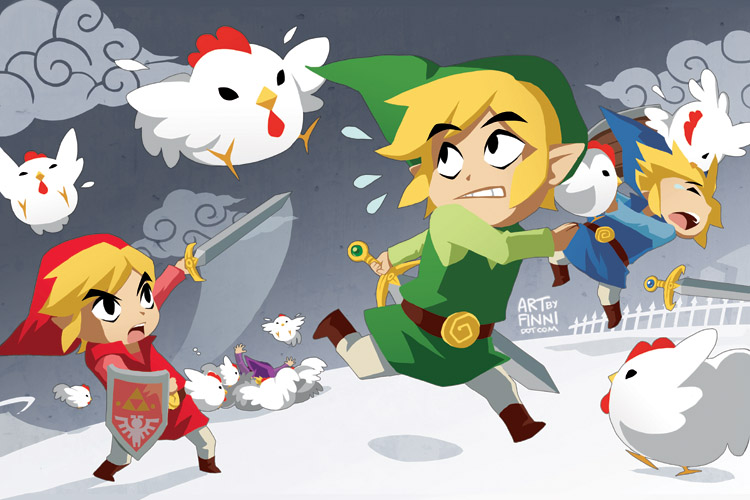
\includegraphics[width=0.6\textwidth]{figures/Sample/tumblr_static_eaceks0rfxsss8o4swscw40wo.jpg}
    \caption[Single Figure Environment Listed Title]{This is a single figure 
    environment}
    \label{fig_singleenv}
\end{figure}

This is a multi-image figure with a top (Figure~\ref{fig_multienv_1}) and bottom (Figure~\ref{fig_multienv_2}) aligned subfigures:

\begin{figure}[ht]
	\centering
	\begin{subfigure}[t]{\textwidth}
		\centering
		
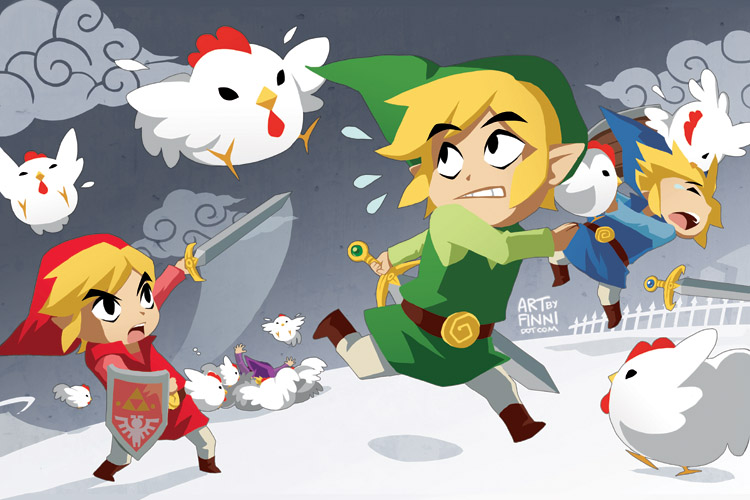
\includegraphics[width=0.7\textwidth]{figures/Sample/tumblr_static_eaceks0rfxsss8o4swscw40wo.jpg}
		\caption{Figure 1}
		\label{fig_multienv_1}
	\end{subfigure}
	~
	\begin{subfigure}[t]{\textwidth}
		\centering
		
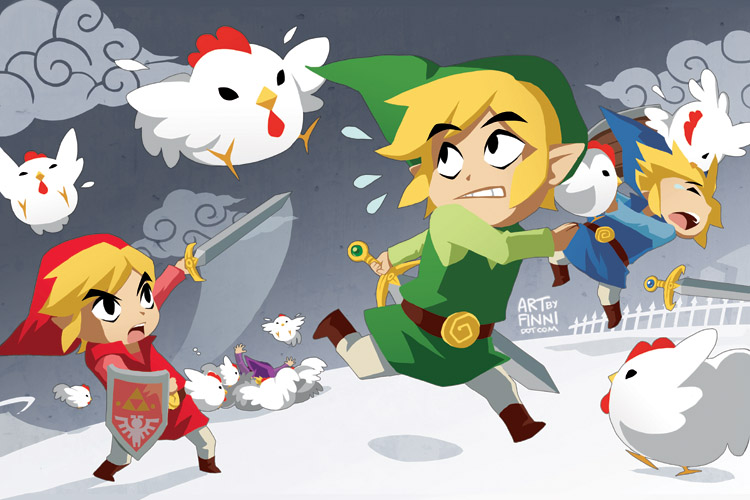
\includegraphics[width=0.7\textwidth]{figures/Sample/tumblr_static_eaceks0rfxsss8o4swscw40wo.jpg}
		\caption{Figure 2}
		\label{fig_multienv_2}
	\end{subfigure}
	
	\caption{A Multi-Figure Environment}
	\label{fig_multienv}
\end{figure}

\section{Tables}

Here is a sample table (Table~\ref{tab_sample}):

	\begin{table}[ht]
	\centering
	\begin{tabular}{ m{0.2\textwidth} m {0.1\textwidth} m{0.15\textwidth} }
		\toprule
		A & $\longleftrightarrow$ & B \\
		C & $\longleftrightarrow$ & D \\
		\bottomrule	
	\end{tabular}	
	\caption{A sample table}	
	\label{tab_sample}
\end{table}

\subsection{Long Tables}
A sample long table is shown in Appendix~\ref{appendix_b}.

\section{Equations}

Here is a sample equation (Equation~\ref{eq_lineslope}):

\begin{equation} \label{eq_lineslope}
	y = mx + b
\end{equation}                  
       \setcounter{figure}{0}
       \setcounter{equation}{0}
       \setcounter{table}{0}

  \chapter{Conclusion}

\section{Referencing}
These are some sample references to GAMYGDALA~\citep{popescu2014gamygdala} from 
the \texttt{references.bib} file and state effects of 
cognition~\citep{hudlicka2002time} from the \texttt{references\_another.bib} 
file. These references are not in the same .bib file.

\section{Figures}
This is a single image figure (Figure~\ref{fig_singleenv}):

\begin{figure}[ht]
    \centering
    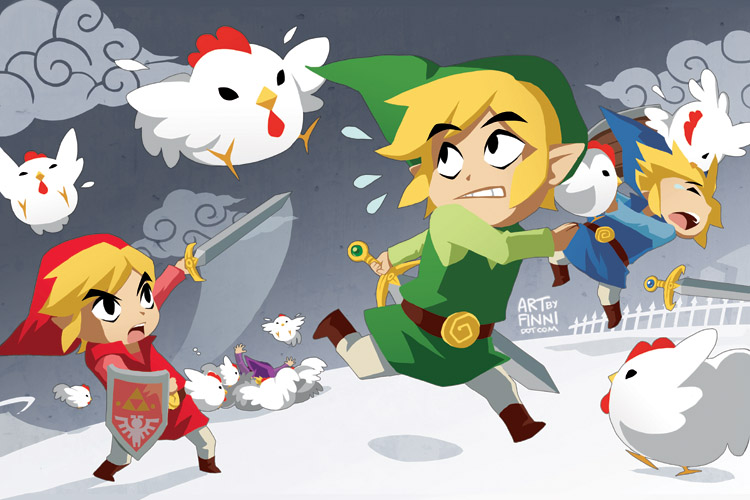
\includegraphics[width=0.6\textwidth]{figures/Sample/tumblr_static_eaceks0rfxsss8o4swscw40wo.jpg}
    \caption[Single Figure Environment Listed Title]{This is a single figure 
    environment}
    \label{fig_singleenv}
\end{figure}

This is a multi-image figure with a top (Figure~\ref{fig_multienv_1}) and bottom (Figure~\ref{fig_multienv_2}) aligned subfigures:

\begin{figure}[ht]
	\centering
	\begin{subfigure}[t]{\textwidth}
		\centering
		
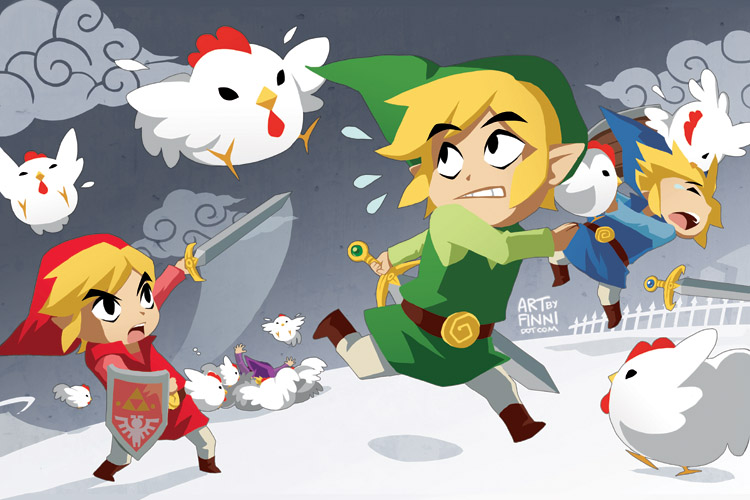
\includegraphics[width=0.7\textwidth]{figures/Sample/tumblr_static_eaceks0rfxsss8o4swscw40wo.jpg}
		\caption{Figure 1}
		\label{fig_multienv_1}
	\end{subfigure}
	~
	\begin{subfigure}[t]{\textwidth}
		\centering
		
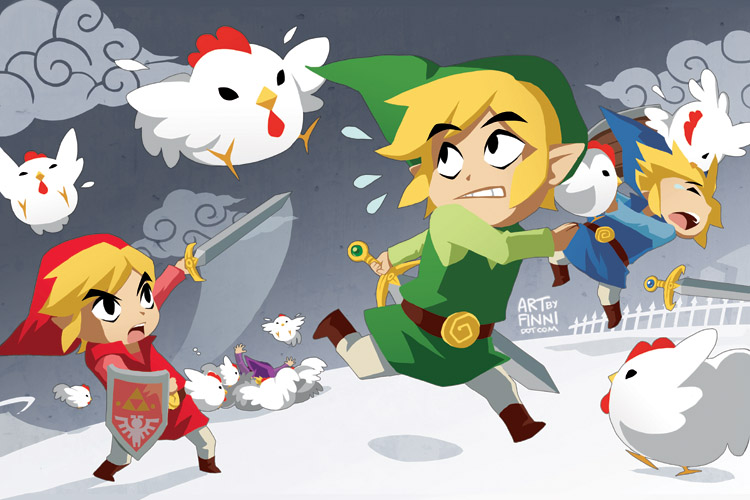
\includegraphics[width=0.7\textwidth]{figures/Sample/tumblr_static_eaceks0rfxsss8o4swscw40wo.jpg}
		\caption{Figure 2}
		\label{fig_multienv_2}
	\end{subfigure}
	
	\caption{A Multi-Figure Environment}
	\label{fig_multienv}
\end{figure}

\section{Tables}

Here is a sample table (Table~\ref{tab_sample}):

	\begin{table}[ht]
	\centering
	\begin{tabular}{ m{0.2\textwidth} m {0.1\textwidth} m{0.15\textwidth} }
		\toprule
		A & $\longleftrightarrow$ & B \\
		C & $\longleftrightarrow$ & D \\
		\bottomrule	
	\end{tabular}	
	\caption{A sample table}	
	\label{tab_sample}
\end{table}

\subsection{Long Tables}
A sample long table is shown in Appendix~\ref{appendix_b}.

\section{Equations}

Here is a sample equation (Equation~\ref{eq_lineslope}):

\begin{equation} \label{eq_lineslope}
	y = mx + b
\end{equation}
        \setcounter{figure}{0}
        \setcounter{equation}{0}
        \setcounter{table}{0}

\begin{appendix}
    \chapter{Your Appendix}
\label{appendix_a}

Your appendix goes here.

        \setcounter{figure}{0}
        \setcounter{equation}{0}
        \setcounter{table}{0}

    \chapter{Scenario Validation}\label{appendix_b}

\sloppy
The images related to scenario validations can be found from the project's Google Drive\footnote {\url{https://drive.google.com/drive/u/1/folders/1uTl1b0Fq_30UqRpwzeT3SyYyPLVKFt__}}. The following table includes the brief details of each image.

\begin{longtable}{|p{0.3\textwidth}|p{0.6\textwidth}|}
\hline
Image Name & Detail \\
\hline
\endfirsthead

\hline
Image Name & Detail \\
\hline
\endhead

\hline
\endfoot

\hline
\endlastfoot

% Data 1 & Data 2 \\

\end{longtable}


        \setcounter{figure}{0}
        \setcounter{equation}{0}
        \setcounter{table}{0}
\end{appendix}

% The bibliography is set up to allow for multiple bib files
\bibliographystyle{ACM-Reference-Format}
\bibliography{references,references_another}

\label{NumDocumentPages}

\end{document}
% ********************************
